% The Introduction should frame the scientific issues that motivate the study. It should briefly indicate the study's objectives and provide enough background information to clarify why the study was undertaken and what hypotheses were tested. An overview of the key publications in the field is essential.
\chapter{Introduction}
\label{sec:introduction}

% - Free Play
Humans are capable of exploring and learning about the world in a self-supervised free-form manner without the presence of explicit predefined goals.
Particularly observable in children, this is a process that is freely chosen and driven by intrinsic motivation, curiosity, and simply the desire to explore and experiment with the environment \citep{seven_play}.

The exact role of such play in human learning is debated across fields.
% It requires an agent to incur extra costs in exploration and can seem counter-intuitive. 
% \todo{Talk more about the importance of free play.}
Yet it has been established as a crucial component for the development of cognitive skills, acquisition of knowledge about the world, and adaptation to new environments \citep{playmontana,playreview}.
% \todo{Talk about the correlation between intelligence acquisition and free play}
As \citet{chu2020play} note, ``...our ability to choose arbitrary costs and rewards allows us to pursue novel goals, discover unexpected information, and invent problems we would not otherwise encounter. Because (predefined) problems impose constraints on search, these invented problems may help solve a big problem: how to generate new ideas and plans in an otherwise infinite search space.''

% \todo{Add more developmental psychology and cognitive science references about creative exploration in children and adults}
This process of \emph{free play} in humans is also characterized by creativity, which is especially apparent in certain forms of play like construction activities.
This involves imagination which allows children to create mental images related to their existing knowledge, feelings, thoughts, and ideas, which they then incorporate into their play \citep{learning_though_play}.
% - Bias towards semantics in cognitive science
Thus, free play is intertwined with visual perception and semantics (meaning), and 
our inherent preferences for visual semantics play a pivotal role in guiding our curiosity-driven exploration, i.e. we constantly seek to understand the semantics of the objects and scenes we encounter based on our prior experiences \citep{exploration}.

% \todo{Characteristics of free play - going to previous biases towards free play}
In a study on free play conducted by \citet{diggs}, in which they asked participants to freely interact with a grid of pixels with no predefined goal or external rewards, both adults and children showed a preference for semantic expression in the form of regular and symmetric patterns that depict real-world objects or concepts (see \figref{fig:diggs}).
% They invent a rich diversity of goals, take costly actions to pursue those goals despite receiving no external rewards,
% and deploy rich planning strategies in the process to achieve this.

This furthers the idea that humans have an innate bias or intrinsic motivation towards visual semantics, i.e. a propensity to explore their environments in expressive styles that manifest their previous knowledge and understanding of the world.
This is related to ``meaningful play'' as defined by \citet{unesco} and particularly present in children as they spend substantial time fiddling with toys, scribbling, and playing with building blocks, meanwhile creating patterns and arrangements that are meaningful to them.

% \vspace{12pt}
\begin{figure}[h]
    \centering
    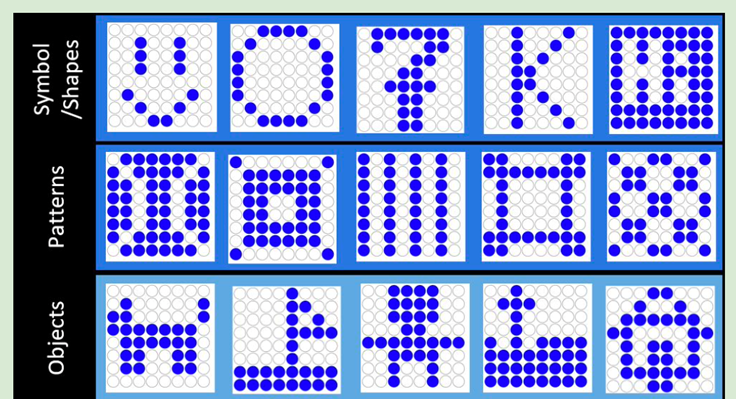
\includegraphics[width=0.7\textwidth]{images/diggs.png}
    \captionsetup{justification=centering}
    \caption[Some creations from the free-play study on humans by \cite{diggs}.]{Some creations from the free-play study on humans by \cite{diggs}.\\(Taken from the original publication.)}
    \label{fig:diggs}
\end{figure}
% \vspace{12pt}

Such play with meaning might serve as a mechanism for the brain to efficiently and quickly learn and adapt to new environments by linking new experiences to existing mental structures and frameworks, i.e. a form of transfer learning.
Indeed, evidence from functional imaging studies in neuroscience shows that meaningful experiences present a blend of familiar and novel stimuli, and recruit a host of neural networks that are involved in novelty processing (medial orbitofrontal cortex), memory (hippocampus), and intrinsic rewards (striatum), which can together be forceful drivers of learning \citep{neuronovel} and building insight \citep{insight}.

% Meaningful experiences present a blend of familiar
% and novel stimuli, initiating neural networks involved
% with novelty processing, memory, and reward seeking
% exploration that are useful in learning (Bunzeck,
% Doeller, Dolan, & Duzel, 2012). Studies demonstrate
% that familiar inputs combined with a novel reward
% can result in stronger hippocampal activity than
% familiar stimuli with familiar reward predicted
% (Bunzeck et al., 2011). 

% Lastly, some evidence tells us that the formation
% of new insights are encoded in our memories by
% activating the brain’s internal reward network
% (Kizilirmak et al., 2016). Involving the intrinsic reward
% system activates the hippocampus, which is useful
% for encoding the meaningful relationship we have
% just acquired, as well as its later retrieval (Kizilirmak
% et al., 2016).

% \todo{Find more references on this bias towards semantics in cognitive science}
% Cedric Collas and Pierre-Yves Oudeyer have some papers on this bias towards semantics in developmental psychology.

\newpage
In the context of artificial intelligence, reinforcement learning (RL) has emerged as a powerful framework for training artificial agents capable of learning complex behaviors (policies) to solve tasks based on the pursuit of rewards through trial and error \citep{sutton2018reinforcement}.
It has shown remarkable success in a wide range of environments.
However, it can require a substantial amount of data to train and has yet to achieve a comparable quality of efficient learning and generalization that humans can achieve through exploration in high-dimensional and complex environments.
Thus scalable and effective exploration remains a fundamental challenge in RL. 
% A fundamental challenge in RL is the trade-off between exploitation (maximizing the expected cumulative rewards) and exploration (gathering information about the environment to improve the policy).
% Exploration is important for an agent to discover enough about its surroundings to be able to ensure optimal policies or internal models that generalize well to unseen states.

% However, most RL algorithms are designed to solve specific tasks and do not consider the free-play exploration paradigm that is of interest to us; they require a specific goal to be achieved, either self-generated or manually defined.

% \todo{Better segregate the different exploration methods (maybe in methods)}
Among the various methods to model exploration in RL, formulations of \emph{intrinsic rewards} \citep{exploration_survey} with curiosity-based \citep{icm,vime}, novelty-based \citep{burda2018largescale,novel_explore}, or uncertainty-based \citep{rnd,plan_explore,disagreement} methods have been proposed to encourage agents to explore their environment in a self-supervised manner. 
% \todo{Play vs exploration}
Yet these methods reward low-level exploration as they are designed explicitly to incentivize maximal information gain for improving internal models and policies.
The precise novelties they promote might not be effectively (semantically) novel and the agent can be stuck in the pursuit of meaningless exploratory goals in an overwhelming search space.
% Consequently, they may not scale to domains requiring more abstract skills.

% which are distinctively marked by the self-governed creation of new goals and rich planning strategies rather than the pursuit of predefined goals in a robotic manner.
% They invent a rich diversity of goals, take costly actions to pursue those goals despite receiving no external rewards,
% and deploy rich planning strategies in the process to achieve this.

This thesis considers the role of our visual semantic priors as abstractions in shaping exploration, embracing the idea that our knowledge and innate visual preferences act as a compass for more efficient and structured high-level exploration during free play by directing our attention and interactions toward semantic expression and discovery.
We imbue artificial agents with this visual semantics bias that emerges and expresses itself automatically as the agent plays freely with the environment, akin to that in humans.

This is done by leveraging large vision language models (VLMs), which are deep neural networks trained on massive generic text and image datasets using the recent advances in self-supervised learning \citep{ssl} and attention architectures \citep{vit}. 
The abstractions of natural language \citep{languageforlearning,vlmhumans}, which reflect the semantics of the world, allow them to learn efficient representations that encapsulate human visual understanding.
% 
% - VLM Applications
Also termed as ``foundation models'', VLMs are capable of transferring to a diverse range of downstream applications beyond visual detection, classification, and object detection.
For example, pre-trained vision-language encoders, such as CLIP \citep{clip}, have successfully been used for image generation \citep{imagegeneration}, decision making \citep{decision_making_clip}, robot control \citep{cliport,embodied}, and more \citep{vlmsurvey}.
% 
% In reinforcement learning, CLIP features have been used to integrate semantic information about the environment in the policy network to improve its perception \citep{vlmcontrol}.
% Pretrained language models can also provide useful initializations for training policies to imitate offline trajectories [42, 27].
% These successes demonstrate that large pre-trained models contain prior knowledge that can be useful for RL. While the existing literature uses pre-trained embeddings directly in the agent, we instead allow the policy network to learn from scratch and only utilize pre-trained embeddings to guide exploration during training (Figure S2).
% 
% - VLM as Rewards
Recent work \citep{zest,negprompt,vlmrm,lamp} has shown that they can also be used as effective abstractions to generate zero-shot rewards for language-guided goal-conditioned tasks in reinforcement learning.

Additionally, VLMs have also been used to improve exploration as tools for refining intrinsic reward signals by abstracting away pseudo-novelty \citep{vlmdistill} or to pursue language-based internally-generated goals \citep{vlmlang}.
% Yet these methods are extensions of the typical intrinsic reward formulations, and like their predecessors, incentivize efficient exploration.
% They do not consider the free-play exploration paradigm that is of interest to us, and require a specific goal to be achieved, either self-generated or manually defined.
Yet these approaches to abstracted exploration do not generate the rich and diverse creative behaviors characteristic of human exploration during play. 

% - Entropy Rewards
Our approach is fundamentally different from these existing studies as we are specifically interested in emergent and creative semantic expression.
We use CLIP to generate exploratory intrinsic rewards that incentivize the agent to freely play in the environment and use its entities to express itself such that a meaningful creation emerges automatically.
This intrinsic reward formulation is based on minimizing the entropy of a VLM's predictions over a set of creative possibilities that the environment offers.
Although the range of freedom is limited to these possibilities, there is no explicit goal specification,
and our controller can exploit this intrinsic entropy reward to guide the agent to any semantically expressive state that the VLM finds confidently meaningful.

We test our formulation in two rich creative environments: the traditional puzzle Tangram and a pixel grid similar to \figref{fig:diggs} and show the limitations of CLIP that pose challenges in shaping our reward.
Subsequently, we introduce several modifications and regularization techniques adapted from previous work on using VLMs as a source of rewards in goal-conditioned tasks to mitigate these limitations and demonstrate their effects in independent ablation studies.
These modifications help the agent to reach a meaningful state, keep it from getting stuck with imperfect creations (false positives or local optima), and improve its exploration to a diverse range of creative possibilities.

% \todo{Comments on shaping of clip rewards near and far from the goal states}
% \todo{Comments on regularization}

% - RaIR (Regularity as Intrinsic Reward)
Furthermore, since there is an implicit order and regularity in meaningful creations, and given the compositional strategies for creative expression learned by humans during early development that favor symmetry \citep{symmetry} and uniformity \citep{compositional}, we hypothesize that a complementary intrinsic reward for this regularity \citep{rair} could promote semantic expression.

With the added bells and whistles, we show that the semantics entropy reward is effective in consistently guiding the agent to discover a range of diverse semantically expressive states in both environments.

% We find that our agent invents a rich diversity of goals despite receiving no external reward, and deploys rich planning strategies in the process.

The work presented in this thesis improves upon and furthers the methods of using VLMs as a source of rewards in reinforcement learning and presents a novel perspective on imbuing human-like free-play behaviors in artificial intelligence with emergent exploration and free-form creativity.
